\chapter{Architektura}
\label{ch:architektura}

W tym rozdziale zostanie omówiona część projektu związana z architekturą systemu, środowiskiem pracy oraz ogólnie przyjętymi rozwiązaniami.

\section{Wiodąca technologia}

Podczas wyboru wiodącej technologii w projekcie wzięto pod uwagę głównie kwestię szybkości dostępu do aplikacji dla użytkowników oraz możliwość jej obsługi na wielu urządzeniach jednocześnie, w tym jako aplikacji desktopowej, mobilnej na system IOS oraz Android. Tym samym, ze względu na rozbudowaną i rozproszoną architekturę, zależało autorowi na jednolitej technologii.

\subsection{Możliwości}
Rozważając decyzję wyboru głównej technologii pod uwagę wzięto 3 podejścia.
\begin{itemize}
    \item \textbf {Aplikacje mobilne w natywnych technologiach} \\
        Wybór budowy natywnych aplikacji mobilnych wiązałby się z tym, że aby utrzymać aplikację dla systemu IOS, Android oraz wersję desktopową wystąpiłaby potrzeba utrzymywania systemu w kilku różnych językach programowania, co znacznie mogłoby obniżyć jakość kodu oraz utrudnić realizację projektu oraz jego dalsze utrzymywanie. Inną wadą tego rozwiązania byłyby płatne i skomplikowane publikacje aplikacji mobilnych. Ostatnim oraz najważniejszym czynnikiem pominięcia wyboru tego rozwiązania był wymagany czas i miejsce w urządzeniu podczas instalacji aplikacji. Ideą aplikacji jest możliwość jej szybkiej instalacji, stąd też na podstawie innych znalezionych rozwiązań, to zostało zdysklasyfikowane mimo możliwości zapewnienia wszystkich natywnych funkcjonalności.

    \item \textbf {Aplikacje mobilne napisane w React Native} \\
        React Native to technologia opracowana przez firmę Facebook w celu przyśpieszenia procesu tworzenia aplikacji mobilnych. Pozwala ona na jednoczesne budowanie aplikacji zarówno na system IOS jak i na Android w języku JavaScript. Mimo zoptymalizowanego procesu budowania aplikacji mobilnych nadal, wedle założeń projektu, potrzebne jest zbudowanie aplikacji desktopowej. Tym samym proces publikacji aplikacji pozostaje dokładnie taki sam jak w pierwszym rozwiązaniu budowy aplikacji w technologiach natywnych.

    \item \textbf {Aplikacja internetowa SPA oraz PWA} \\
        Ostatnią braną pod uwagę możliwością była aplikacja internetowa typu SPA omówiona w rozdziale Frontend w sekcji React \ref{ch:frontend:react} razem z PWA, omówiona w sekcji PWA \ref{ch:frontend:pwa}. Takie podejście umożliwia budowę szybkiej oraz wieloplatformowej aplikacji w jednolitej technologii oraz architekturze. Użytkownicy posiadają dostęp do strony internetowej, która może zostać zainstalowana na każdym telefonie oraz komputerze znacznie szybciej oraz zajmuje mniejszą ilość miejsca na urządzeniu niż w przypadku natywnych technologii. Mimo ograniczenia niektórych funkcjonalności, szczególnie na telefonach z systemem IOS, względem natywnych rozwiązań wybrane podejście oferuje funkcjonalności potrzebne do budowy projektu. Kolejną rzeczą, która zadecydowała o wyborze był proces publikacji aplikacji. Rozwiązanie to pozwala na jednoczesną, prostą i bezpieczną publikację w jednolitym systemie.
\end{itemize}

\subsection{Wybór}
Ze względu na szybkość dostępu, łatwość instalacji z punktu widzenia użytkowników, jednolitą technologię dla wielu platform oraz prostszy w porównaniu\newline z pozostałymi możliwościami proces publikacji, ostatecznym wyborem pozostała aplikacja internetowa typu SPA oraz PWA.

\section{JavaScript}
Jako główny język programowania wykorzystany do implementacji tego projektu został zastosowany JavaScript. Ze względu na swoje możliwości oraz szeroką społeczność, umożliwia on jednoczesną budowę wszystkich części projektu (klient, serwer, raspberry pi).

JavaScript (JS) jest skryptowym oraz dynamicznym językiem programowania wysokiego poziomu stworzonym przez firmę Netscape. Jego bezpośrednim twórcą jest amerykański programista Brendan Eich. JavaScript jest wieloparadygmatowym językiem programowania co oznacza, że można w nim programować zarówno obiektowo, funkcyjnie jak i imperatywnie. Wersje JavaScriptu rozpoznawane są względem standardu specyfiki ECMAScript wydaną przez organizację ECMA. Obecnie rozwojem tego standardu zajmuje się komicja TC39, która zrzesza przedstawicieli wszystkich głównych przeglądarek internetowych. \cite{JavaScriptBasics} Według ogólnoświatowej ankiety z 2020 roku portalu StackOverflow, język JavaScript został określony jako najpopularniejsza technologia, dokładnie 69,7 procent respondentów dokonało takiego wyboru. \cite{StackOverflowSurvey}

Ważnym aspektem wersji tego języka jest jego wspieranie w różnych przeglądarkach. Tworząc nowy projekt chcemy korzystać zazwyczaj z najnowszych implementacji przy jednoczesnej obsłudze w różnych przeglądarkach i ich różnych wersjach. Jako rozwiązanie tego problemu powstał darmowy i otwarty transpilator JavaScriptu. Umożliwia on konwersję z najnowszych wersji JS do tego zgodnego z ES5 (wersja JS z 2009 roku przyjęta jako minimalny standard użycia).

\section{Stos technologiczny}
Ze względu na zakres projektu i umożliwienie jak najprostszej dalszej rozbudowy projektu oraz doświadczenie komercyjne autora w budowaniu aplikacji internetowej wybrano stos technologiczny zwany MERN (MongoDB-Express-React-Node). Technologie z wybranego podejścia MongoDB, Express oraz Node zostały opisane w rozdziale \ref{ch:backend} - Backend oraz React w rozdziale \ref{ch:frontend} - Frontend.

\section{Diagram klas}
Diagram klas obejmujący wszystkie encje w systemie został zilustrowany przez rysunek \ref{fig:ClassDiagram} oraz \ref{fig:AbstractClassDiagram}. Wszystkie przedstawione encje posiadają pole \textit{BaseField}, które przedstawia unikalne id, datę utworzenia i modyfikacji. Każdy zespół, posiada swoją nazwę, jednego lub dwóch graczy oraz tablice indykującą aktualnie zaproszonych graczy. Gracz oraz administrator zawierają podstawowe pola użytkownika \textit{User} w tym: dane służące autentykacji, email, hasło, aktualny status (w zależności od potwierdzenia konta mailowego lub odrzucenia przez administratora). Klasa \textit{Player}, reprezentująca gracza, posiada pola dodatkowe względem administratora, w tym: imię, nazwisko, region użytkownika oraz awatar. Każda notyfikacja w systemie przypisana jest do konkretnego gracza. Zapisywane w systemie gry posiadają zawsze dwa zespoły, pole wygranego zespołu, swój status aktywności, pole określające czas nagrywania powtórek oraz miniony czas meczu. Gole natomiast przypisane są zawsze do konkretnej gry oraz posiadają one id zespołu, który strzelił gola oraz link do wideo powtórki.

\begin{figure}[h!]
    \centering
    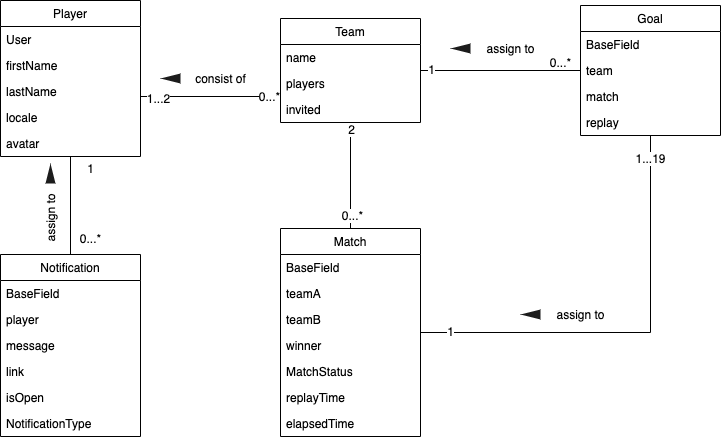
\includegraphics[width=0.8\textwidth]{images/diagrams/class_diagram.png}
    \caption{Diagram klas z asocjacjami}
    \label{fig:ClassDiagram}
\end{figure}

\begin{figure}[h!]
    \centering
    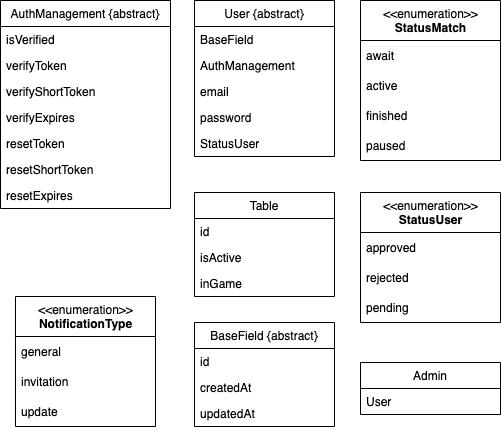
\includegraphics[width=0.6\textwidth]{images/diagrams/class_diagram_rest.png}
    \caption{Diagram klas abstrakcyjnych oraz klas bez relacji}
    \label{fig:AbstractClassDiagram}
\end{figure}

\section{Struktura projektu}
Ze względu na fakt budowy wielu serwisów, które mogą dzielić między sobą zasoby oraz potrzebują siebie nawzajem do prawidłowego działania, projekt wymagał narzędzia, które umożliwi dynamiczną pracę miedzy pakietami. Podczas planowania struktury i przyszłego zarządzania projektem wzięto pod uwagę 3 podejścia. W każdej z przedstawionych możliwości założono wykorzystanie narzędzia kontroli wersji \textit{git} oraz menadżera zależności \textit{Yarn}.

\begin{itemize}
    \item \textbf {Osobne repozytoria z wykorzystaniem yarn link} \\
        Pierwszym rozważanym podejściem było stworzenie osobnych repozytoriów dla każdego z pakietów.
        Umożliwiłoby to zachowanie klarownej historii repozytorium dla każdego pakietu. W przypadku osobnych repozytoriów, korzystanie przez siebie nawzajem byłoby możliwe z wykorzystaniem komendy `yarn link` między pakietami. Takie rozwiązanie jednakże byłoby problematyczne przy pracy, ze względu na ilość pakietów oraz dlatego, że komendę odpowiadającą za linkowanie między pakietami trzeba byłoby wpisywać z każdą reinstalacją zależności w pakietach. Innym problem dla takiego podejścia byłaby konfiguracja narzędzi takich jak linter czy prettier, ponieważ ich konfiguracje musiałyby się znaleźć w każdym z repozytorium a zmiany wprowadzone w jednym miejscu trzeba byłoby nanosić manualnie w innych miejscach. \cite{YarnLinkDocs}

    \item \textbf {Osobne repozytoria z wykorzystaniem git submodules} \\
        Innym podobnym rozwiązaniem, do tego powyższego, byłoby zastosowanie git submodules. Umożliwiłoby to utrzymywanie każdego serwisu w osobnym repozytorium, ale całość połączona miałaby swoje repozytorium z odnośnikami do poszczególnych repozytoriów. Rozwiązałoby to kwestie globalnej konfiguracji narzędzi takich jak linter ale nadal pozostałby problem z wzajemnym linkowaniem między serwisami. \cite{GitSubmodulesDocs}

    \item \textbf {Monolityczne repozytorium z wykorzystaniem yarn workspaces} \\
        Ostatnią rozważaną możliwością była budowa projektu jako jednego monolitycznego repozytorium. To rozwiązanie wprowadza pojęcie paczek, które w powyższych opcjach byłyby osobnymi repozytoriami. Dzięki takiemu podejściu możemy przechowywać cały projekt w jednym repozytorium, jednakże zmniejsza to czytelność historii komitów repozytorium. Mimo wymienionej wady zarządzanie oraz korzystanie z projektu w tym przypadku może być znacznie prostsze. Korzystając z workspace'ów wszystkie paczki mogą, bez żadnej dodatkowej konfiguracji, korzystać z siebie nawzajem. Poza tym globalna konfiguracja narzędzi takich jak linter jest możliwa dla wszystkich paczek. \cite{YarnWorkspacesDocs}

\end{itemize}

Ostatecznym wyborem pozostało podejście budowy projektu w architekturze monolitycznego repozytorium korzystając z yarn workspaces.

\newpage

\section{Struktura pakietów}
Ze względu na wybraną strukturę projektu mono repozytorium wszystkie aplikacje zostały zaimplementowane w jednym repozytorium i podzielone na siedem oddzielnych pakietów. Cała struktura pakietów została przedstawiona na ilustracji \ref{fig:packages-structure}. Każdy z pakietów został dokładnie opisany w rozdziale \ref{ch:application}.

\begin{figure}[h!]
  \centering
    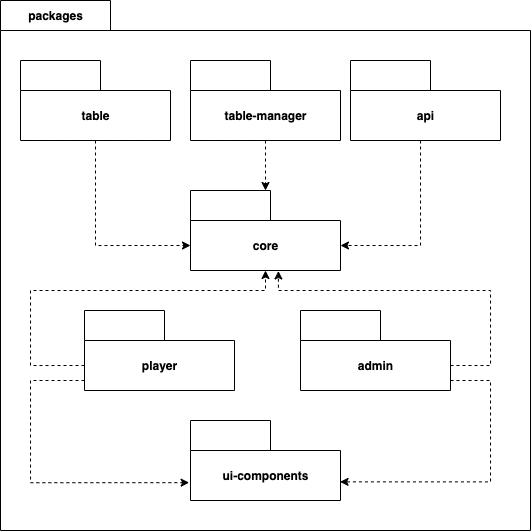
\includegraphics[width=0.7\textwidth]{images/diagrams/packages_structure.png}
  \caption{Struktura pakietów}
  \label{fig:packages-structure}
\end{figure}


\section{Typy}
Język JavaScript jest językiem programowania, który nie jest silnie typowany. Ze względu na rozmiar całego systemu oraz brak możliwości typowania w wybranym języku programowania, został przygotowany pakiet 'core', który podzielony jest na dwie części, tj. modele oraz stałe.
Dzięki takiemu rozwiązaniu zostało wprowadzone ręczne typowanie części logiki biznesowej całego systemu oraz stałych zmiennych wykorzystywanych we wszystkich pakietach poprzez zwykłe obiekty. 

Innym narzędziem rozwiązującym problem braku typowania jest paczka 'Prop Types' pochodząca od twórców biblioteki 'React'. W projekcie wykorzystywana jest w pakietach 'player', 'admin' oraz 'ui-components'. Jej zadaniem jest kontrola typów przyjmowanych argumentów w komponentach graficznych.

Dzięki dwóm powyższym rozwiązaniom budowa aplikacji posiada rodzaj mechanizmu typowania. Przyczynia się to do szybszego procesu pracy oraz zmniejsza ilość potencjalnych błędów w systemie.

\section{Środowisko developerskie}
Podczas wyboru technologii oraz narzędzi do pracy bardzo ważnym etapem był dobór środowiska developerskiego. Przez środowisko developerskie rozumiane są narzędzia służące ogólnej pracy nad programistyczną częścią systemu, zwiększeniu jej bezpieczeństwa oraz jej przyśpieszeniu.

\subsubsection{Edytor kodu}
Przy budowie systemu, wybranym edytorem kodu źródłowego został program 'Webstorm' firmy Jetbrains. Głównym przeznaczeniem tego edytora są aplikacje pisane w języku JavaScript. W przeciwieństwie do innych programów przeznaczonych do edycji kodu, jego skupienie się na jednym obszarze implikuje wiele wbudowanych narzędzi wspierających ten język programowania. Poniżej opisane narzędzia posiadają wbudowaną integrację z edytorem, przez co praca z nimi staje się jeszcze prostsza. Innym czynnikiem decydującym o wyborze tego edytora było doświadczenie biznesowe oraz projektowe autora systemu. W tym przypadku doświadczenie w korzystaniu z tego typu narzędzia pełni bardzo dużą rolę pod względem znajomości skrótów klawiszowych, które pozwalają na znaczne przyśpieszenie pracy oraz na skupienia się na realnych problemach ponad powtarzającymi się operacjami.


\subsubsection{Menadżer Wersji Node}
Kolejnym narzędziem, które pozwoliło na ułatwienie pracy jest menadżer wersji Node - 'NVM' (Node Version Manger).
Pozwala on na dynamiczne przełączanie się i szybką instalację różnych wersji. Środowisko uruchomieniowe Node, które wykorzystywane jest w projekcie, jest bardzo dynamicznie rozwijającą się platformą. Z każdą wersją staje się ono znacznie bezpieczniejsze oraz szybsze. Istnieją jednak biblioteki oraz narzędzia, które wymagają użycia specyficznych \newline i starszych wersji Node. Rozwiązaniem problemu potrzeby częstego przełączania się pomiędzy wersjami w celu testowania bibliotek oraz częstej aktualizacji do najnowszych wersji jest właśnie NVM. \cite{NVMDocs}

Przykładowo w celu szybkiej instalacji oraz przełączenia się na 12 wersje Node wystarczy w konsoli wpisać: 'nvm install 12'. W przypadku kiedy w systemie posiadamy zainstalowaną już wersje 12 i chcemy się tylko na nią przełączyć wystarczy wpisać: 'nvm use 12'. Również kiedy, tak jak w omawianym systemie, użytkownik w głównym katalogu projektu będzie posiadał plik '.nvmrc' z numerem minimalnie wymaganej wersji Node, komenda 'nvm use', automatycznie zainstaluje wskazaną wersję.


\subsubsection{Lintery}
W cały projekcie zostały zastosowane różnego rodzaju lintery, czyli narzędzia służące unifikacji kodu, utrzymywaniu dobrych praktyk notacji oraz innych opisów.

Najważniejszym ze wszystkich linterów jest Eslint, który na wywołanie komendy lub zapis dowolnego pliku w projekcie (dzięki integracji z edytorem kodu) dokonuje statycznej analizy kodu według zasad określonych w pliku konfiguracyjnym (.eslintrc). Zastosowany w projekcie plik konfiguracyjny został oparty głównie o zestaw zasad używanych przez firmę Airbnb. Firma ta udostępnia darmową bibliotekę, która umożliwia proste zamontowanie jej z pliku konfiguracyjnym. W notacji narzędzia Eslint omawiany system rozszerza zestaw zasad Airbnb oraz nadpisuje zaledwie małą część zadeklarowanych zasad na potrzeby wymagań projektu.

Drugim, w kolejności najważniejszym linterem jest Prettier, który działa w bardzo podobny sposób co Eslint. Skupia się on jednak na analizie stylu kodu źródłowego w przeciwieństwie do Eslinta, który skupia się na składni języka i bibliotek. Przykładowymi elementami kodu, na których skupia się Prettier jest długość linii lub odstępy między nawiasami.

Obydwa powyżej opisane lintery oferują możliwość automatycznego formatowania według ustalonych zasad. Dzięki takiej formie auto-formatowania programista mógłby napisać nawet całą klasę, składającą się z wielu metod i pól w jednej linii, a wspomniane dwa lintery przy zapisaniu pliku sformatowałyby klasę do czytelnej formy według ustalonych zasad. Ze względu na architekturę systemu mono repozytorium, każdy z pakietów posiada swój własny plik konfiguracyjny, który rozszerza globalny zadeklarowany plik w katalogu głównym. Takie podejście pozwala na proste zarządzanie plikami konfiguracyjnymi, a w przypadku potrzeby zmian zasad per pakiet, programista może zmienić zasady w wybranej konfiguracji nie zmieniając przy tym pozostałych pakietów.

Trzecim linterem jest 'Commitlint', który odpowiada za walidację opisów komitów w gicie. Wybrana konfiguracja implementuje specyfikację Convetional Commits. W przypadku, kiedy wiadomość będzie niezgodna ze specyfikacją, użytkownik uzyska błąd oraz komit nie zostanie wysłany. Takie podejście oferuje spójną historię wiadomości komitów w gicie oraz możliwość automatycznego wygenerowania przy użyciu dodatkowych narzędzi pliku graficznego opisującego zmiany od ostatniej publikacji.

Ostatnim linterem jest paczka sort-package-json, która pozwala na sortowanie plików package.json w projekcie. Uruchomienie sortowania odbywa się poprzez wpisanie komendy 'yarn sortPackageJson' w terminalu znajdując się w głównym katalogu projektu. 

\subsubsection{Zarządzanie mono-repozytorium}
Narzędziem, które w projekcie zostało zastosowane do zarządzania \break mono-repozytorium jest biblioteka 'lerna'. Pozwala ona na wiele czynność dotyczących pracy z tym rodzajem repozytorium. Jest to narzędzie, które współpracuje z klientem NMP (node package manager) co oznacza, że może tak jak NMP zarządzać zależnościami. Konfiguracja tego narzędzia znajduje się w katalogu głównym w pliku 'lerna.json'. Funkcjonalności lerny, jakie wykorzystywane są w systemie to deklaracja zależności, które mają być unikalne w konkretnym pakiecie, uruchamianie skryptów we wszystkich pakietach jedną komendą oraz dodawanie zależności per pakiet lub do wszystkich pakietów na raz.

\subsubsection{Scripty}
Nawiązując do poprzednio omawianej funkcjonalności lerny, odnośnie uruchamiania skryptów dla wszystkich pakietów do zarządzania powtarzającymi się skryptami, zostało użyte jeszcze jedno narzędzie. 'Scripty' to paczka, która umożliwia uruchamianie wszystkich wykonywalnych skryptów w plikach package.json. Dzięki temu skrypty, które uruchamiane są w każdym z pakietów (posiadając taką samą konfigurację) mogą zostać wydzielone do osobnego folderu. Przy dodawaniu nowych skryptów należy jednak pamiętać o nadawaniu praw odczytu/zapisu. W tym celu najlepiej jest skorzystać ze stworzonego skryptu poprzez wywołanie komendy 'yarn grant-scripty-permissions' w terminalu znajdują się w głównym folderze. Komenda ta nadaje wymagane prawa dla wszystkich skryptów znajdujących się w folderze 'scripts'. Warto mieć na uwadze, że prawa dla dodanych skryptów będą zapisane w historii gita, dlatego też operacja ta wymagana jest tylko jednorazowo dla każdego nowego skryptu.

\subsubsection{Zarządzanie wersją}

Praca programistów niezależnie od języka programowania, wiąże się z dużą ilością pracy oraz potrzebą zmian wraz z rozwojem projektów, co w efekcie potrafi powodować wiele problemów. Rozwiązaniem na to są systemy zarządzania wersją. W omawianym projekcie wybrany został system 'git'. Tego rodzaju zarządzanie wersjami pozwala na dowolne przełączanie się pomiędzy wcześniej wysłanymi zmianami, przez co programista jest w stanie wrócić w każdym momencie w bardzo szybki sposób do poprzednich wersji, nie tracąc przy tym też obecnie rozwijanej. Narzędzie te posiada wbudowaną integrację z wybranym edytorem kodu 'Webstorm' przez co używanie tego rozwiązania jest intuicyjne dzięki wbudowanemu interfejsowi graficznemu. Poza wspomnianym zarządzaniem wersjami, system ten pozwala na budowę różnych funkcjonalności w separacji dzięki tzw. gałęziom (branches). Każda zmiana wymaga utworzenia tzw. komitu, który zatwierdza zmiany i montuje je w aktualnie wybranej lub wskazanej gałęzi.
W połączeniu z wcześniej omówionym narzędziem commitlint w sekcji lintery, narzędzie to jest w stanie tworzyć pewnego rodzaju dokumentację. Zakładając używanie poprawnej notacji wiadomości komitów, użytkownik w historii komitów będzie widział jasno udokumentowaną historię zmian.

Git oferuje również system tzw. hooków czyli mechanizmów, które pozwalają na wpięcie się w cykl życia różnych wywoływanych funkcji gita.\cite{GitHooksDocs} Dodatkowym narzędziem, zastosowanym w projekcie, który wykorzystuje wspomnianą funkcjonalność jest husky. Dzięki temu, skrypty takie jak wspomniany eslint, prettier czy commitlint mogą być uruchamiane automatycznie podczas wywoływania wybranych git hooków. W połączeniu z huskym została również zastosowana paczka 'lint-staged', która w przypadku użycia eslint oraz prettier w git hookach, sprawdza tylko pliki, które zostały zmienione od ostatniego komita, dzięki czemu analiza kodu jest dokonywana znacznie szybciej.

\subsubsection{Zdalne repozytorium}

Kolejną rzeczą w kontekście zarządzania wersją jest Github, serwis hostingowy przeznaczony dla repozytoriów z systemem git. Serwis ten powstał w 2008 roku oraz obecnie rozwijany jest przez firmę Microsoft.\cite{GithubWiki} Z punktu widzenia zarządzania projektem (nie tylko programistycznego), jest to idealne oraz główne miejsce służące do przechowywania plików projektowych oraz kopii. Kod źródłowy omawianego projektu przechowywany jest właśnie za pomocą serwisu Github. Utrzymując projekt w sieci programiści, w połączeniu z systemem git, mają możliwość synchronicznej pracy nad jednym projektem oraz zunifikowany dostęp do projektu z każdego miejsca na świecie. Github posiada również wbudowane narzędzie 'Github Actions', które umożliwia uruchamianie zadeklarowanych skryptów w języku yaml podczas tworzenia Pull Requestów. Pull Requesty są funkcjonalnością opcjonalną w pracy z tym narzędziem, jednak wysoko zalecanym wedle standardów projektowych. Pozwalają one na zebranie w jednym miejscu podsumowania wszystkich komitów, które można połączyć z wybraną gałęzią w gicie. Takie podsumowanie umożliwia również wyświetlenie informacji o statusie działania wspomnianych 'Github Actions' w kontekście nowo stworzonego pull requesta.